\section{Estado del arte: ciencia de los datos}
\label{sec:state_dataScience}

\subsection{Introducción}
\label{subsec:state_dataScience_intro}

Las bases de datos NoSQL no son lo único que ha traído el ``Big Bang'' de la
información en Internet. Igual que se hace evidente la necesidad de
poder almacenar toda ésta nueva información de manera eficiente, también lo hace
la necesidad de aprovechar y utilizar éstos datos de manera eficiente. A éstos
efectos, se ha ido gestando una nueva disciplina dedicada al estudio de nuevos métodos para generar información útil a partir de datos de
cualquier manera, a la que hoy se conoce como ``ciencia de los datos'', o en
inglés, \emph{data science}.

El primer uso del término data a 1966 cuando Peter Naur utilizó en 1966
porque no le gustaba el nombre de  ``ciencias de la computación'', y consideraba
este último más apropiado. Incluso hoy en día, aunque el término lleve usándose en su forma actual más de veinte
años, no existe ninguna definición formal sobre qué entraña exactamente, sino
que simplemente diferentes investigadores han aportado su opinión en
qué quiere decir el término. Chikio Hayashi (\cite{Hayashi1998}) la definió como
\emph{un concepto para unificar estadística, análisis de datos y métodos
  relacionados}, y Zhu et. al (\cite{Zhu2011}) la definieron de forma elegante
como \emph{una nueva ciencia cuyo objeto de estudio son los datos}. 


\subsection{Flujo de trabajo}
\label{subsec:state_dataScience_workflow}

Dentro de un proyecto de análisis de datos, existen una serie de pasos que en
conjunto, forman una manera de trabajar que, aún sin existir un consenso sobre
qué trata la ciencia de los datos, se ha estandarizado:

\begin{figure}[ht!]
  \centering
  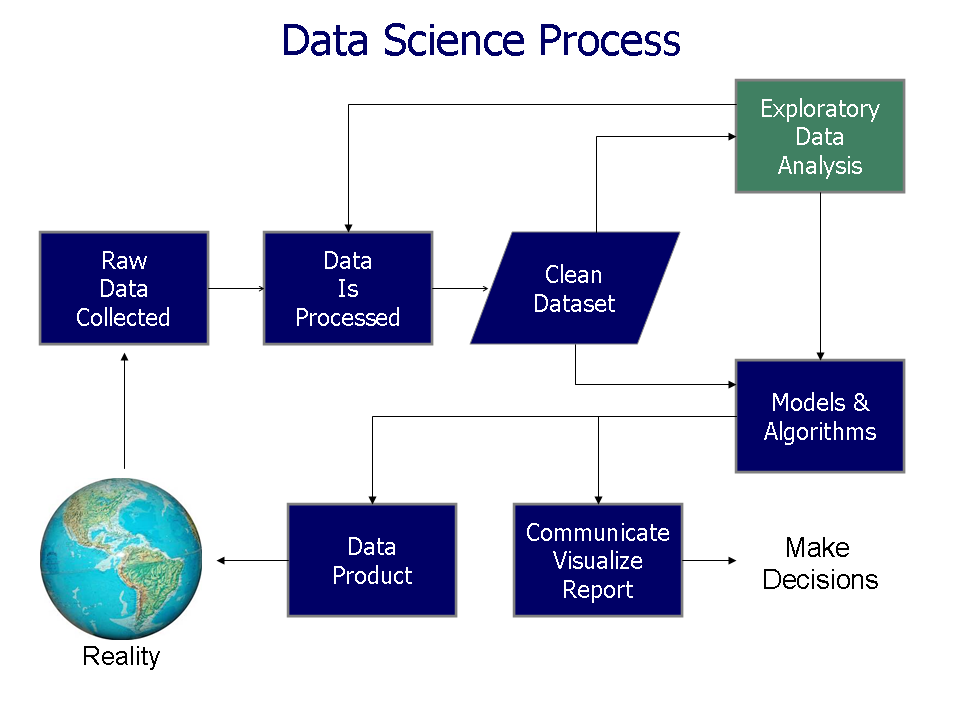
\includegraphics[scale = 0.65]{img/data_science_process.png}
  \caption{\label{fig:dataScienceWorkflow} Flujo de trabajo del científico de datos}
\end{figure}


\subsubsection{Formulación de la hipótesis}
\label{subsec:state_dataScience_workflow_1}

Al inicio del proyecto, nos encontramos ya de entrada con una decisión
importante. ?`Qué es lo que queremos investigar? ?`Con qué objetivo?

Cada empresa tiene sus necesidades específicas, y opera en un mercado
determinado. Por tanto, resulta importante que el científico de datos sepa
formular una pregunta u hipótesis, que al ser respondida con el análisis, genere
algún valor para la empresa. Para ello conviene tener conocimientos de dominio
(\emph{domain knowledge} en inglés), en otras palabras, conocer medianamente
el entorno en el que se generan los datos, y la información / fenómenos que describen.

\subsubsection{Obtención de los datos}
\label{subsec:state_dataScience_workflow_1}

Una vez ha definido la pregunta a responder, es hora de obtener los
datos. Éstos pueden venir de una infinidad de fuentes o formatos de fichero:
desde CSV, hojas de cálculo de Excel o LibreOffice y ficheros en formato JSON /
XML, a bases de datos relacionales y NoSQL. La siguiente tabla muestra la lista
de métodos de los que dispone Pandas (una librería para Python que provee
estructuras de datos y herramientas para facilitar el análisis) para leer
fuentes de datos, y generar un DataFrame (una estructura de datos tabular):

\begin{table}[h!]
\centering
\label{pandas_readData}
\begin{tabular}{|l|l|}
\hline
\textbf{Método} & \textbf{Fuente de datos}                                  \\ \hline
read\_csv       & Fichero CSV                                               \\ \hline
read\_excel     & Hoja de cálculo de Excel                                  \\ \hline
read\_hdf       & Fichero HDF (Formato de datos jerárquico)                 \\ \hline
read\_sql       & Base de datos relacional                                  \\ \hline
read\_json      & Fichero o cadena JSON                                     \\ \hline
read\_msgpack   & Formato de serialización msgpack                          \\ \hline
read\_html      & Tablas dentro de ficheros HTML                            \\ \hline
read\_gbq       & Google BigQuery                                           \\ \hline
read\_stata     & Ficheros DTA de Stata                                     \\ \hline
read\_sas       & Ficheros de SAS                                           \\ \hline
read\_clipboard & Contenidos del portapapeles a través de read\_table       \\ \hline
read\_pickle    & Estructuras de datos guardadas mediante el formato pickle \\ \hline
\end{tabular}
\caption{Métodos de Pandas para leer datos}
\end{table}

Obviamente, existen muchos más formatos en los que podemo encontrar los datos,
a parte de los que Pandas puede leer. En ese caso, tocará recurrir a otras
herramientas con las que podamos interactuar con el servicio en
cuestión, para posteriormente transferir los datos a un DataFrame, o cualquier
otra estructura que deseemos utilizar.

% TODO: Hablar un poco sobre la minería de datos.

\subsubsection{Limpieza y preparación de los datos}
\label{subsec:state_dataScience_workflow_1}

Una vez ya hemos importado los datos, y los estamos manipulando con el lenguaje
de nuestra elección, debemos echarle un vistazo general al dataset, y ver si
observamos alguna anomalía.

En pandas, la clase DataFrame dispone de algunos métodos bastante interesantes
para ver rápidamente algunos registros del dataset: 

\vspace{0.5cm}

\begin{TMcode}{Python}{}{Bloque de código}
accidents_2015 = pd.read_csv("data/ACCIDENTS_GU_BCN_2015.csv", encoding="latin1", delimiter=";")

accidents_2015            # Muestra el dataset en su totalidad
accidents_2015.head()     # Muestra los 5 primeros registros
accidents_2015.tail()     # Muestra los 5 últimos registros
accidents_2015.sample(15) # Muestra 15 registros aleatorios
\end{TMcode}
\vspace{1cm}

Por ejemplo, si ejecutamos \texttt{accidents\_2015.head()}, en una libreta de
Jupyter veremos lo siguiente:

\begin{figure}[ht!]
  \hspace{-0.7cm}
  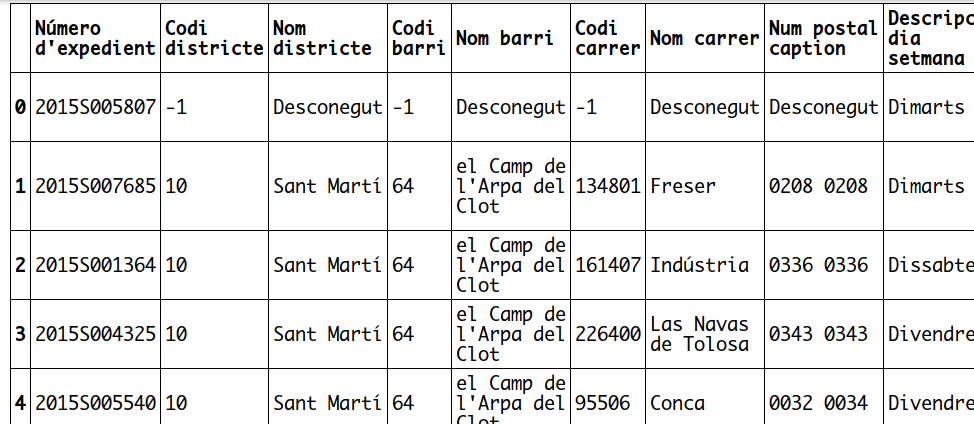
\includegraphics[scale = 0.45]{img/dataframeHead.png}
  \caption{\label{fig:dataframeHead} Dataframe.head() en Jupyter Notebook}
\end{figure}

Básicamente, las preguntas que deberíamos tratar de responder con éste análisis
inicial son las siguientes:

\begin{enumerate}
\item Existe alguna anomalía en los datos? Falta algún valor?
\item Observamos algún patrón en los datos?
\end{enumerate}


\paragraph{Trabajando con valores faltantes} \mbox{}\\

En caso de que en nuestro dataset nos encontremos con variables para las que
directamente no exista una observación, existen varias técnicas que podemos
utilizar para tratar los registros.

Las dos primeras que describiremos, trabajan de forma destructiva, es decir,
borrando datos: 

\begin{TMbulletin}{critical}{$¡$Cuidado!}
  Al borrar / ignorar la informacion faltante, éstos métodos pueden
  introducir \textbf{imparcialidad estadística}.
\end{TMbulletin}
\footnote{Se da cuando
el resultado obtenido difiere del verdadero parámetro siendo estimado.}

\begin{enumerate}
\item Borrar por completo cada registro en el que falte alguna observación
\item Ignorar observaciones faltantes, y realizar análisis únicamente sobre
  aquellas observaciones que sí se encuentren en el dataset.
\end{enumerate}

La otra manera de tratarlos recibe el nombre de \textbf{imputación}, y consiste
en sustituir los valores nulos. Para ésto, también disponemos de varias técnicas:

\begin{enumerate}
\item Para variables contínuas, podemos sustituir valores nulos por la media
  aritmética de los valores no nulos.
\item Para variables categóricas, podemos sustituir valores nulos por la moda de
  los valores no nulos. El valor que más veces se dé, será el que utilizaremos
  en la imputación.
\end{enumerate}


\paragraph{\emph{Tidy data}}\mbox{}\\

Aunque lo ideal sería que cada dataset que encontráramos viniera ya en un
estado ideal para ponernos a analizar su contenido, esto generalmente no es así.
Hadley Wickham utiliza el término \emph{tidy data} (\cite{tidy-data}), para
referirse a cualquier dataset que reúne las siguientes características:

\begin{figure}[ht!]
  \begin{enumerate}
  \item Cada variable es una columna.
  \item Cada observación es una fila.
  \item Cada unidad observacional o entidad forma una tabla.
  \end{enumerate}
  \caption{\label{fig:tidy-data-characteristics} Características de un
    dataset ``limpio''}
\end{figure}

Según Wickham ésta es la tercera forma normal de Codd, con las restricciones
extrapoladas a lenguaje estadístico, y enfocada a un único dataset / tabla, en
lugar de datasets interconectados en una base de datos relacional.

En pandas, podemos utilizar los métodos \texttt{Pandas.pivot()} y
\texttt{Pandas.melt()} para realizar las tareas de ``derretido'' y ``apilado'',
que Wickham describe en el mismo artículo: 

\vspace{0.5cm}

\begin{TMcode}{Python}{}{}
import pandas as pd
df = pd.DataFrame({'Id': {0: 'David', 1: 'b', 2: 'c'},
                   'Lotería': {0: 'Juan', 1: 3, 2: 5},
                   'Sorteo iPad': {0: 'Sergio', 1: 4, 2: 6}})
\end{TMcode}
\vspace{1cm}

Visionando el DataFrame resultante mencionado el valor a secas, obtenemos lo siguiente: 

\begin{table}[ht!]
\centering
\caption{My caption}
\label{my-label}
\begin{tabular}{|l|l|l|l|}
\hline
           & \textbf{Id} & \textbf{Lotería} & \textbf{Sorteo iPad} \\ \hline
\textbf{0} & David           & 0          & 2          \\ \hline
\textbf{1} & Juan            & 3          & 4          \\ \hline
\textbf{2} & Sergio          & 5          & 6          \\ \hline
\end{tabular}
\end{table}

Observando el dataset, aunque sea de ejemplo, podemos ver que incumple uno de
los tres principios del \emph{tidy data}, que cada columna represente una
variable. En éste caso, cada una describe un valor. Entonces,
para transformar el dataset, en un formato más cómodo de trabajar para el
análisis, utilizaremos  \texttt{melt()}: \vspace{1cm}

\begin{TMcode}{Python}{}{}
import pandas as pd

pd.melt(df, id_vars=['Id'], value_vars=['Lotería', 'Sorteo iPad'],
        var_name='Concurso', value_name='VecesGanado')

\end{TMcode}
\vspace{1cm}

\begin{table}[ht!]
\centering
\caption{Dataset derretido}
\label{dataset-derretido}
\begin{tabular}{|l|l|l|l|}
\hline
           & \textbf{Id} & \textbf{Sorteo} & \textbf{Veces Ganado} \\ \hline
\textbf{0} & David       & Lotería         & 0                     \\ \hline
\textbf{1} & Juan        & Lotería         & 3                     \\ \hline
\textbf{2} & Sergio      & Lotería         & 5                     \\ \hline
3          & David       & Sorteo iPad     & 2                     \\ \hline
4          & Juan        & Sorteo iPad     & 4                     \\ \hline
5          & Sergio      & Sorteo iPad     & 6                     \\ \hline
\end{tabular}
\end{table}

El método \texttt{melt}, transforma un dataset en un formato ``ancho'', y apila
sets de variables en únicamente dos columnas: Una representando el nombre de la
variable, y la otra, el valor de la misma. Una vez tenemos el dataset de ésta
manera, resulta mucho más sencillo realizar operaciones cómo por ejemplo ver los
resultados de la lotería, o gente que haya ganado un concurso más de 5 veces:

% TODO: Añadir imágenes del resultado
\begin{TMcode}{Python}{}{Filtrado booleano en Pandas}
  df[df['Concurso'] == 'Lotería']
  df[df['VecesGanado'] > 5]
\end{TMcode}

\subsubsection{Análisis explorativo}
\label{subsec:state_dataScience_workflow_2}

En realidad, el preparado del dataset, y lo que se denomina análisis explorativo
(cuyo propósito es familiarizarnos mejor con el mismo), van bastante unidos de la mano en
el sentido de que para poder corregir anomalías en el dataset, debemos verlo
bien de cerca. De todas maneras, en Pandas disponemos de muchísimos más métodos
de los que hemos visto antes para conocer más de cerca el dataset:


\begin{figure}[ht]
  \centering
  \begin{TMcode}{Python}{}{Análisis explorativo con Pandas}

    DataFrame.shape   # Devuelve las dimensiones (Filas x Columnas)
    DataFrame.columns # Devuelve las columnas (features)
    DataFrame.info    # Devuelve la cantidad de valores no-nulos en cada columna
    DataFrame.describe() # Agregado de estadísticas como la media, min / max, etc...

    DataFrame['VariableCategórica'].unique() # Devuelve la lista de valores que toma la variable.
  \end{TMcode}
  \caption{\label{fig:pandasExplorative} Análisis explorativo con pandas, parte 1}
\end{figure}

Llegados a éste punto, en el que hemos identificado la variable en cuestión como
categórica, es necesario cambiarle el tipo a la misma de cara a la
representación que Pandas hace de la misma:


\vspace{0.5cm}
\begin{TMcode}{Python}{}{}
  df['VariableCategórica'] = df['VariableCategórica'].astype('category')
\end{TMcode}

\vspace{0.5cm}

Una vez hecho ésto, podemos ver la distribución de valores de la variable:

\vspace{0.5cm}
\begin{TMcode}{Python}{}{}
  df['VariableCategórica'].value_counts()
\end{TMcode}


\subsubsection{Visualización de datos}
\label{subsec:state_dataScience_dataVisualization}

Otra parte muy importante que va de la mano con el análisis explorativo, es
generar gráficos que nos ayuden a entender de manera visual, diferentes aspectos
sobre el dataset. Aspectos muy importantes como cualquier patrón, variación
estacional en series de tiempo y correlación, suelen estar ocultos en los
números, y los gráficos son una buena manera de hacerlo. 

Para mostrar ejemplos de éstos gráficos, utilizaremos un dataset de la
temperatura media diaria del río Fisher, cerca de Dallas, de enero de 1998 a
diciembre de 1991:

\vspace{0.5cm}
\begin{TMcode}{Python}{}{}
import pandas as pd
import numpy as np
import matplotlib.pyplot as plt
import matplotlib
%matplotlib inline # Necesario para que Jupyter muestre las figuras en la misma página
matplotlib.style.use('ggplot')
\end{TMcode}

\begin{TMcode}{Python}{}{}
df = pd.read_csv('fisher.csv', delimiter=',', parse_dates=[0], index_col = 0)
\end{TMcode}
\vspace{0.5cm}

Antes de proseguir, es importante destacar los dos últimos parámetros que le
hemos pasado a \texttt(read\_csv): \texttt(parse\_dates) y \texttt(index\_col). En
conjunto, éstos harán que el primer campo del dataset, que es la
fecha, actúe como índice, permitiéndonos hacer cosas como la siguiente:

\vspace{0.5cm}
\begin{TMcode}{Python}{}{}
  df['1990'].plot(figsize=(15, 5)) # Muestra únicamente el año 1990
\end{TMcode}

\begin{figure}[ht]
  \centering
  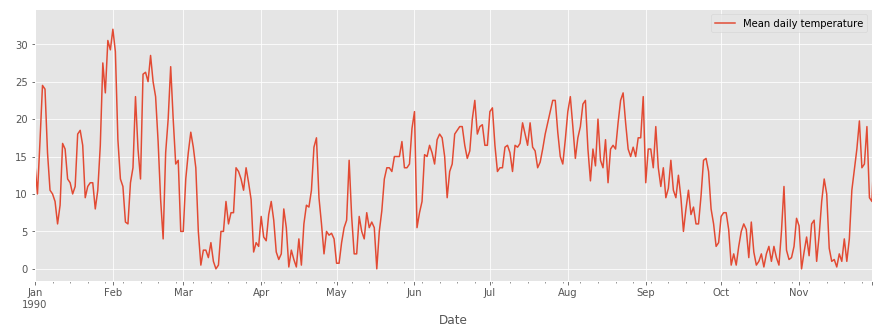
\includegraphics[scale=0.50]{img/yearPlot.png}
  \caption{\label{fig:yearPlot} Temperaturas media diaria del río Fisher a su
    paso cerca de Dallas en el año 1990}
\end{figure}

\subsubsection{Modelado}
\label{subsec:state_dataScience_workflow_modeling}

Un modelo estadístico es una clase específica de modelo matemático, una
manera formal de describir sistemas mediante conceptos matemáticos.

Generalmente, un modelo estadístico implica dos tipos de variables: dependientes
y explicativas:

\begin{itemize}
\item \textbf{Variable dependiente: } se dice de aquella que queremos estudiar o
  predecir. Suele ser aquella que se representa en el eje de las Y.

\item \textbf{Variable explicativa: } También llamadas independientes, son aquellas en las que nos apoyamos para
  describir las variables dependientes.
\end{itemize}

Existen infinidad de modelos estadísticos que tienen en cuenta tanto el tipo de
las variables, como el número de éstas. Uno de los más simples de entender y
implementar es la regresión lineal, empleada para estudiar la relación de
dependencia entre una variable dependiente $Y$, una o más variables
independientes $X_i$, y un término aleatorio $\epsilon$. Si se utiliza una única
variable independiente $X$, hablamos de una regresión linear simple.


\paragraph{Teoría de la regresión linear simple}\mbox{}\\

La ecuación que describe la recta de regresión es: 

\begin{equation}
  Y_i = \beta_0 + \beta_i X_i + \epsilon_i
\end{equation}

Dónde:

\begin{itemize}
\item $\hat{Y}$ es el valor a predecir
\item $\beta$ es la pendiente de la recta
\item A es el punto de intersección en el eje de las Y.
\end{itemize}

La ecuación para la pendiente es:

\begin{equation}
  \beta = r s \frac{\overline{x} * \overline{y} - \overline{xy}}{(\overline{x})^2 - \overline{x^2}}
\end{equation}

Mientras que la del punto de la intersección es:

\begin{equation}
A = M_y - bM_x
\end{equation}

\paragraph{Implementando la regresión lineal simple}\mbox{}\\

En los siguientes bloques de código se demuestra la implementación de una
regresión lineal simple en Python. Para éste ejemplo, estamos utilizando otro
dataset nuevo, que simula el gasto mensual de una persona teniendo en cuenta sus
ingresos y la cantidad de viajes que realiza:

\vspace{0.25cm}
\begin{TMcode}{Python}{}{}
import pandas as pd
import numpy as np

import matplotlib
import matplotlib.pyplot as plt

from sklearn import linear_model, model_selection
from sklearn.metrics import mean_squared_error
%matplotlib inline
matplotlib.style.use('ggplot')
\end{TMcode}
\vspace{0.25cm}

\begin{TMcode}{Python}{}{}
df = pd.read_csv("data/monthlySpending.csv")
df.info()
\end{TMcode}
\vspace{0.25cm}

\begin{TMcode}{Python}{}{}
# Gráfico izquierdo
plt.scatter(df['M_INC'], y)
plt.title("Gasto mensual vs ingresos mensuales")
plt.xlabel("Ingresos mensuales")
plt.ylabel("Gasto mensual")

# Gráfico derecho
plt.scatter(df['M_TRP'], y)
plt.title("Gasto mensual vs viajes mensuales")
plt.xlabel("Viajes realizados")
plt.ylabel("Gasto mensual")
\end{TMcode}
\vspace{0.25cm}

\begin{figure}[h!]
    \centering
    \begin{subfigure}{0.5\textwidth}
    \centering
        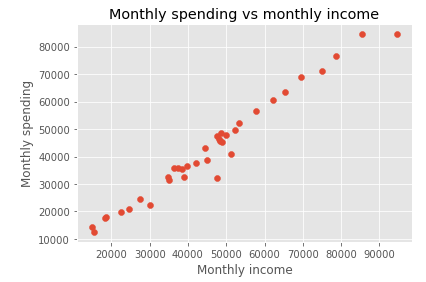
\includegraphics[width=1\linewidth]{img/MspendMinc.png}
        \caption{inclusions}
        \label{fig:inclu}
    \end{subfigure}%
    \begin{subfigure}{0.5\textwidth}
    \centering
        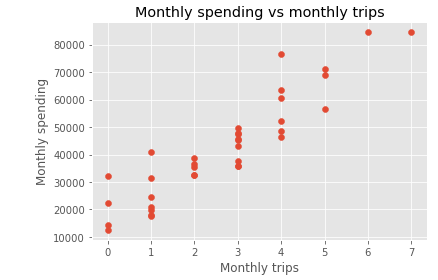
\includegraphics[width=1\linewidth]{img/MspendMtrp.png}
        \caption{grain deformation}
        \label{fig:deform}
    \end{subfigure}
    \caption{filler text}
    \label{fig:manmade}
    \end{figure}
\vspace{0.50cm}

En el siguiente bloque definimos nuestras variables, tanto dependientes (el
gasto mensual), como independientes (el número de viajes, o los ingresos). 

\begin{TMcode}{Python}{}{}
y = df['M_SPEND']
X = df['M_TRP']
\end{TMcode}
\vspace{0.25cm}

\begin{TMcode}{Python}{}{}
linearRegression = linear_model.LinearRegression()

X_train, X_test, y_train, y_test = model_selection.train_test_split(X, y,
test_size = 0.33)

linearRegression.fit(X_train, y_train)
\end{TMcode}
\vspace{0.25cm}

Merece la pena explicar la segunda instrucción, \texttt{train\_test\_split()}.
Éste método se utiliza para dividir nuestras variables en dos datasets cada una,
uno que se utilizará para entrenar el algoritmo, y el otro para comprobar el
mismo una vez entrenado. Ésto se hace debido a que la regresión daría una
precisión del 100\% si lo probamos con los mismos datos con los que lo
entrenamos.

Una vez ya entrenado el clasificador, podemos obtener las métricas de regresión: 

\begin{TMcode}{Python}{}{}
print('Root mean squared error: %.2f ' % math.sqrt(mean_squared_error(reg.predict(X_test), y_test)))
print('Variancia explicada: %.2f' % explained_variance_score(reg.predict(X_test), y_test))
print('Coeficiente de determinación: %.2f' % r2_score(reg.predict(X_test), y_test))
\end{TMcode}
\vspace{0.25cm}

Interpretadas tal que:

\begin{itemize}
\item Cada punto se aleja de media en 2077 unidades de la línea de mejor ajuste
  (\emph{Root mean squared error})
\item Variancia
\item El coeficiente de determinación, también escrito como $R^2$, indica la
  proporción de la variancia en la variable dependiente que es predecible de la
  variable independiente. En otras palabras, estima cuán bien la recta de
  regresión se ajusta a los datos reales. El valor va de 0 a 1, donde un 1
  indica un ajuste perfecto.
\end{itemize}

Una vez verificado el modelo, podemos visualizar la recta de regresión junto a
los \emph{datapoints} con el siguiente bloque de código:

\begin{TMcode}{Python}{}{}
  plt.scatter(X, y)
  plt.plot(X, np.poly1d(np.polyfit(X, y, 1))(X), color='blue')
  plt.xlabel('Monthly trips')
  plt.xlabel('Monthly spending)
\end{TMcode}
\vspace{0.25cm}

\begin{figure}[ht]
  \centering
  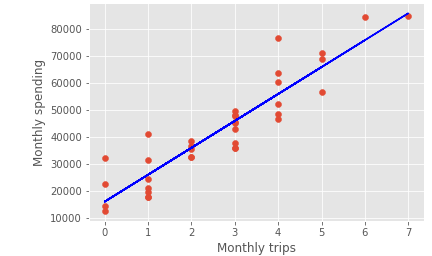
\includegraphics[scale=0.65]{img/bestFitLine.png}
  \caption{\label{fig:bestFitLine} Recta de regresión}
\end{figure}


\subsubsection{Comunicación de los resultados}
\label{subsec:state_dataScience_workflow_communication}

Cuando ya se ha configurado el modelo, y se han obtenido resultados adecuados,
es hora de hacérselos llegar a aquellos que realmente toman las decisiones en la
empresa. El problema es que generalmente, es una audiencia muy diferente

\paragraph{Producto de datos}
\mbox{}\\






